% IEEE conference version for GTSD 2026 proceedings
\documentclass[conference]{IEEEtran}
\usepackage{cite}
\usepackage{amsmath,amssymb,amsfonts}
\usepackage{graphicx}
\graphicspath{{figures/}}
\usepackage{textcomp}
\usepackage{booktabs}
\usepackage{algorithm}
\usepackage{algpseudocode}
\usepackage{url}
\def\BibTeX{{\rm B\kern-.05em{\sc i\kern-.025em b}\kern-.08em
    T\kern-.1667em\lower.7ex\hbox{E}\kern-.125emX}}

\begin{document}
\bstctlcite{IEEEexample:BSTcontrol}

\section{Proposed Hardware-Software Co-Design Framework}

% =========================================================================
% III-A. OVERALL SYSTEM ARCHITECTURE & CO-DESIGN WORKFLOW
% =========================================================================
\subsection{Overall System Architecture and HW/SW Co-Design Workflow}

Deploying deep super-resolution models on resource-constrained edge modalities presents a fundamental architectural dilemma: general-purpose embedded CPUs lack the parallel arithmetic throughput required for real-time 2D convolutions, whereas purely autonomous FPGA implementations suffer from severe development overhead regarding peripheral interfacing, file I/O, and dynamic memory orchestration. To overcome these constraints, we establish a balanced, end-to-end hardware-software co-design architecture deployed on the heterogeneous Xilinx Zynq-7020 System-on-Chip (SoC). As illustrated in Fig.~\ref{fig:sw_hw_architecture}, the system is partitioned into two synchronized computing domains across distinct clock regimes: (1) the software-driven \textbf{Processing System (PS)} running at 650~MHz, and (2) the custom pipelined \textbf{Programmable Logic (PL)} streaming accelerator core operating at a deterministic clock rate of 100~MHz.

\begin{figure*}[t]
\centering
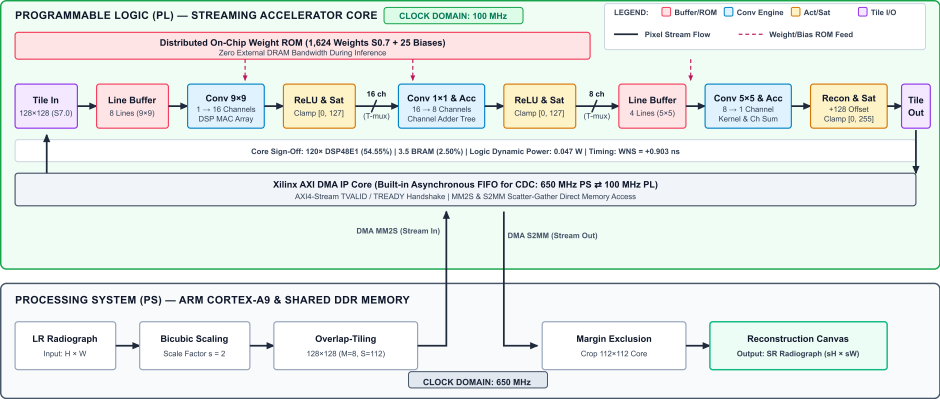
\includegraphics[width=\textwidth]{SW-HW_architeture.jpg}
\caption{End-to-end heterogeneous hardware-software co-design architecture: (1) Processing System (PS) domain running on dual-core ARM Cortex-A9 (650~MHz) for bicubic scaling, overlap-tiling partitioning ($128 \times 128$, $M=8, S=112$), margin exclusion, and final frame stitching, and (2) Programmable Logic (PL) streaming accelerator core (100~MHz) incorporating on-chip distributed weight ROM (1,624 weights S0.7 + 25 biases), 2D line buffers, parallel DSP MAC arrays, and pipelined channel adder trees, interfaced via Xilinx AXI DMA with built-in asynchronous FIFO clock-domain crossing (CDC).}
\label{fig:sw_hw_architecture}
\end{figure*}

\subsubsection{Processing System (PS) Workflow: Pre-Processing and Canvas Reconstruction}
The Processing System (PS), powered by a dual-core ARM Cortex-A9 processor running at 650~MHz under the embedded Linux/PYNQ environment, coordinates high-level medical radiograph management, coordinate geometry transformations, and DMA buffer allocation:
\begin{itemize}
    \item \textbf{Bicubic Scaling:} Given an input low-resolution (LR) radiograph $I_{LR} \in \mathbb{R}^{H \times W}$, the host CPU executes software-based bicubic interpolation by an upscaling factor of $s = 2$, mapping the image onto the target high-resolution (HR) spatial grid ($2H \times 2W$). This pre-upsampling establishes a spatially uniform dataflow for subsequent convolutional stages.
    \item \textbf{Overlap-Tiling Partitioning:} To accommodate the limited on-chip memory budget of edge FPGAs, the interpolated frame is partitioned into overlapping tiles of dimension $P \times P = 128 \times 128$ pixels, using an effective core stride of $S = 112$ and a boundary margin of $M = 8$. Each patch is formatted into signed 8-bit fixed-point representation (S7.0, range $[-128, 127]$).
    \item \textbf{Margin Exclusion and Stitching:} Once super-resolved tiles return from the hardware accelerator, the PS software pipeline discards the $M = 8$ exterior border pixels affected by valid convolution boundary shrinkage, isolating the artifact-free $112 \times 112$ core ($T_{valid}$). The valid cores are subsequently stitched into a continuous reconstruction canvas to reconstruct the full diagnostic radiograph ($I_{SR} \in \mathbb{R}^{sH \times sW}$).
\end{itemize}

\subsubsection{Clock-Domain Crossing and AXI DMA IP Interconnect}
Data interchange between the 650~MHz Processing System and the 100~MHz Programmable Logic fabric is arbitrated by an on-chip \textbf{Xilinx AXI Direct Memory Access (AXI DMA) IP Core}. The DMA controller bridges the two asynchronous clock domains using built-in asynchronous dual-clock FIFOs, completely eliminating metastability risks and clock-domain crossing (CDC) penalties. Utilizing high-throughput 64-bit AXI High-Performance (HP) ports, the DMA engine performs bidirectional Scatter-Gather streaming:
\begin{itemize}
    \item \textbf{DMA MM2S Channel (\textit{Memory-Mapped to Stream}):} Reads contiguous S7.0 input tile buffers directly from off-chip DDR3 DRAM and streams them into the accelerator's AXI4-Stream Slave port under standard \texttt{TVALID}/\texttt{TREADY} flow control.
    \item \textbf{DMA S2MM Channel (\textit{Stream to Memory-Mapped}):} Captures the super-resolved output stream from the accelerator's AXI4-Stream Master port, automatically transferring completed frames into destination memory upon detecting the asserted \texttt{TLAST} packet boundary flag.
\end{itemize}

\subsubsection{Programmable Logic (PL) Streaming Accelerator Datapath}
The custom hardware accelerator instantiated on the Artix-7 logic fabric of the Zynq-7020 executes the entire 3-layer compact SRCNN inference pipeline in a continuous streaming manner at 100~MHz:
\begin{itemize}
    \item \textbf{Distributed On-Chip Weight ROM:} All 1,624 quantized convolutional weights (signed S0.7) and 25 biases are pre-loaded into distributed on-chip ROM blocks directly adjacent to the compute cores. This architectural choice achieves \textit{zero external DRAM memory bandwidth during active inference}, entirely circumventing the von Neumann memory wall.
    \item \textbf{Layer 1 (Patch Extraction \& Feature Representation):} Streaming S7.0 pixels pass through an 8-line 2D line buffer (BRAM-based shift registers) that reconstructs a full $9 \times 9$ spatial sliding window on every clock cycle. The $9 \times 9$ convolution engine employs a parallel DSP MAC array to project the single input channel into 16 intermediate feature maps ($1 \rightarrow 16$), followed by a parametric ReLU and saturation unit that clamps activations into $[0, 127]$. The resulting 16 channels are time-multiplexed (\textit{T-mux}) into the next stage.
    \item \textbf{Layer 2 (Non-linear Mapping):} A $1 \times 1$ convolution engine paired with a balanced, pipelined channel adder tree compresses the 16 feature maps into 8 channels ($16 \rightarrow 8$). Activations are clamped via a second ReLU and saturation stage before being time-multiplexed into the final reconstruction layer.
    \item \textbf{Layer 3 (High-Resolution Reconstruction):} The 8-channel activations enter a 4-line buffer to form a $5 \times 5$ sliding window. The $5 \times 5$ convolution engine ($8 \rightarrow 1$) computes both spatial kernel products and multi-channel accumulations concurrently. The final Reconstruction \& Saturation block adds a $+128$ offset to de-quantize signed intermediate values back to standard unsigned uint8 representations ($[0, 255]$), streaming the super-resolved tile out via the AXI4-Stream Master interface.
    \item \textbf{Hardware Sign-Off Summary:} The accelerator core achieves complete timing closure with a positive Worst Negative Slack of $\text{WNS} = +0.903$~ns at 100~MHz, while consuming merely 120 DSP48E1 slices (54.55\% of budget), 3.5 BRAM blocks (2.50\%), and dissipating an ultra-low logic dynamic power of only 0.047~W.
\end{itemize}

The subsequent subsections detail the mathematical formulation of the compact network topology (Section~\ref{sec:topology}), the fixed-point quantization scheme (Section~\ref{sec:quantization}), the boundary-safe overlap-tiling strategy (Section~\ref{sec:tiling}), and the internal microarchitectural timing closure (Section~\ref{sec:rtl_arch}).

% =========================================================================
% III-B. COMPACT SRCNN NETWORK TOPOLOGY & TRAINING PROTOCOL
% =========================================================================
\subsection{Compact SRCNN Network Topology and Pre-Quantization Training}
\label{sec:topology}
% Outline & Key Concepts:
% 1. Architectural Justification: Custom 3-layer lightweight CNN (1 -> 16 -> 8 -> 1) with kernel sizes 9-1-5, totaling only 1,624 weights and 25 biases (1,649 parameters), compared to standard SRCNN's 8,032 parameters.
% 2. Mathematical Definition of Layers:
\begin{equation}
F_l(Y) = \max\left(0,\, W_l * F_{l-1}(Y) + B_l\right), \quad l \in \{1, 2\}
\label{eq:srcnn_relu}
\end{equation}
\begin{equation}
F_3(Y) = W_3 * F_2(Y) + B_3
\label{eq:srcnn_linear}
\end{equation}
% - Layer 1 (Extraction): 9x9 kernel, Cin=1, Cout=16 + ReLU.
% - Layer 2 (Non-linear Mapping): 1x1 kernel, Cin=16, Cout=8 + ReLU.
% - Layer 3 (Reconstruction): 5x5 kernel, Cin=8, Cout=1, linear output to preserve radiological dynamic range and avoid clipping negative residual values.
% 3. Pre-Quantization Training Protocol:
%    - Training Dataset: 15,000 radiograph patches (size 64x64 extracted from clinical medical training sets).
%    - Objective Loss: Charbonnier/L1 loss to penalize high-frequency edge deviations without over-smoothing.
%    - Optimizer & Schedule: Adam optimizer (initial lr=1e-3, cosine decay, 50 epochs), providing high-fidelity FP32 baseline (39.31 dB PSNR) prior to quantization.
% 4. Figure Placeholder: Fig. 3 (Detailed layer-by-layer tensor dimensions, channel widths, and receptive field expansion).

% =========================================================================
% III-C. FIXED-POINT MATHEMATICAL FORMULATION & POST-TRAINING QUANTIZATION
% =========================================================================
\subsection{Fixed-Point Mathematical Formulation and Post-Training Quantization (PTQ Q7)}
\label{sec:quantization}
% Outline & Key Concepts:
% 1. Motivation: Complete elimination of floating-point arithmetic units (FPU) to maximize logic density and energy efficiency on Zynq-7020.
% 2. Data Format Definition:
%    - Pixel Activations: Signed S7.0 (1 sign bit, 7 integer bits, 0 fractional bits, range [-128, 127]).
%    - Model Weights: Signed S0.7 (1 sign bit, 0 integer bits, 7 fractional bits, range [-1.0, +0.992]).
% 3. Mathematical Quantization Equations:
\begin{equation}
X^{(0)}(i, j) = \text{clamp}\left(I_{in}(i, j) - 128,\, -128,\, 127\right)
\label{eq:input_quant}
\end{equation}
\begin{equation}
W_q = \text{clamp}\left(\left\lfloor W \cdot 2^7 \right\rceil,\, -128,\, 127\right)
\label{eq:weight_quant}
\end{equation}
\begin{equation}
A_k(i, j) = \sum_{c=0}^{C_{in}-1} \sum_{u=0}^{K-1} \sum_{v=0}^{K-1} X_c(i+u, j+v) \cdot W_{k,c}(u, v) + \left(B_k \ll 7\right)
\label{eq:mac_accumulation}
\end{equation}
\begin{equation}
X_k^{(l)}(i, j) = \min\left(\max\left(0,\, \left\lfloor A_k(i, j) \gg 7 \right\rfloor\right),\, 127\right), \quad l \in \{1, 2\}
\label{eq:layer_activation}
\end{equation}
\begin{equation}
I_{out}(i, j) = \min\left(\max\left(0,\, \left\lfloor A_3(i, j) \gg 7 \right\rfloor + 128\right),\, 255\right)
\label{eq:output_dequant}
\end{equation}
% 4. Critical Binary Point Alignment Insight:
%    - Product of (S7.0) * (S0.7) produces S7.7 (7 fractional bits).
%    - Bias B_k (originally S7.0) must be bit-shifted left by 7 bits (B_k << 7) in Eq. (5) to align binary points before accumulation.
%    - Intermediate accumulators sized to 24-bit to prevent any arithmetic overflow across large 9x9 summation trees.
%    - Re-quantization via arithmetic right-shift (>> 7) in Eq. (6) and saturation clamping to prevent wrap-around distortions.

% =========================================================================
% III-D. HARDWARE-AWARE OVERLAP-TILING & BOUNDARY ARTIFACT ELIMINATION
% =========================================================================
\subsection{Hardware-Aware Overlap-Tiling and Boundary Artifact Elimination}
\label{sec:tiling}
% Outline & Key Concepts:
% 1. Problem: Arbitrary large radiograph resolutions (1024x1024 to 2048x2048) far exceed FPGA on-chip BRAM capacity (140 BRAM blocks).
% 2. Receptive Field & Valid Core Derivation:
\begin{equation}
R = 1 + \sum_{l=1}^3 (K_l - 1) = 1 + (9-1) + (1-1) + (5-1) = 13\text{ pixels}
\label{eq:receptive_field}
\end{equation}
\begin{equation}
M_{min} = \left\lceil \frac{R - 1}{2} \right\rceil = 6\text{ pixels} \quad \Longrightarrow \quad \text{Select } M = 8\text{ pixels}
\label{eq:margin}
\end{equation}
% 3. Grid Partitioning & Canvas Dimensions (Complete Closed-Form Formulas):
\begin{equation}
N_R = \left\lceil \frac{sH}{S} \right\rceil, \quad N_C = \left\lceil \frac{sW}{S} \right\rceil
\label{eq:tile_grid}
\end{equation}
\begin{equation}
H_{pad} = N_R \cdot S + 2M, \quad W_{pad} = N_C \cdot S + 2M
\label{eq:canvas_pad}
\end{equation}
%    - Constants: Scale s=2, Tile size P=128, Core stride S=112, Margin M=8 (P = S + 2M = 112 + 16 = 128).
% 4. True Exterior Image Boundary Handling (Edge-Replication Padding):
%    - At the true image perimeter where no adjacent tiles exist, replicate border pixels (mode='edge') into the outer margin:
%      I_pad(x, y) = I_bic(clamp(x, 0, sW-1), clamp(y, 0, sH-1)).
%    - Completely eliminates boundary blocking artifacts, step discontinuities, and artificial border seams.
% 5. Algorithm Placeholder: Algorithm 1 (Hardware-Aware Overlap-Tiling and DMA Streaming Execution).

% =========================================================================
% III-E. STREAMING RTL ACCELERATOR MICROARCHITECTURE (ZYNQ-7020 PL)
% =========================================================================
\subsection{Streaming RTL Accelerator Microarchitecture}
\label{sec:rtl_arch}
% Outline & Key Concepts:
% 1. 2D Line-Buffer Design:
%    - BRAM-based shift-register cascade caching K-1 rows per convolutional stage.
%    - Enables single-port continuous streaming from AXI-Stream while presenting a full K x K sliding kernel to the compute datapath every single clock cycle.
%    - Minimal memory footprint: Consumes only 3.5 BRAM36K blocks (2.50% of the 140 available budget).
% 2. Parallel MAC Array & DSP48E1 Mapping:
%    - Hardware mapping: Exploits signed 8-bit integer multipliers mapped directly into Xilinx DSP48E1 slices.
%    - Resource-efficient allocation: Exactly 120 DSP48E1 slices utilized (54.55% of the 220 budget), leaving ample logic margin for system peripherals.
% 3. Pipelined Balanced Adder Tree:
%    - Multi-stage reduction tree processing all spatial products concurrently with registered pipeline stages, guaranteeing optimal timing slack.
% 4. Clock Domain & 100 MHz Timing Closure:
%    - Fully synchronous single-clock domain (100 MHz) spanning AXI-Stream master/slave interfaces, line buffers, and compute array.
%    - Eliminates asynchronous FIFO clock-domain crossing (CDC) latency and area penalties.
% 5. Latency & Deterministic Throughput:
%    - Sustained throughput of 1 output pixel per clock cycle without pipeline stalls.
%    - End-to-end latency: 6.33 ms per 128x128 tile, delivering 157.9 patches/s sustained accelerator throughput.
% 6. Figure Placeholder: Fig. 6 (Microarchitectural schematic: Line buffer chain, sliding window registers, DSP MAC array, adder tree, saturation shifters, and AXI4-Stream FSM).

\bibliographystyle{IEEEtran}
\bibliography{bib/references}
\end{document}
